\begin{abstract}
We present a systematic framework for studying LLM sycophancy. We distinguish two elicitation regimes: \textbf{context-induced sycophancy}, where user framing already invites accommodation in the first response, and \textbf{trigger-induced sycophancy}, where unsupported social pressure is applied after an initial answer. \ourWork focuses primarily on the trigger-induced regime. It is a principled benchmark grounded in social psychology that frames each item as a decision-support problem and decomposes the benchmark design into three layers: \textbf{context}, \textbf{trigger}, and \textbf{multi-turn progression}. It also provides a reusable toolbox of social-pressure triggers that can be applied to existing benchmarks. Across XXX items spanning four domains (STEM, Health \& Medicine, Social Science, and Humanities), we instantiate eight families of unsupported social-pressure cues, including a mechanism-free simple baseline, and model how pressure unfolds through simple repetition, combined-trigger trajectories, escalation, and de-escalation.
Second, \textbf{SycoScope} offers a toolbox to detect sycophantic behavior by methods of mechanistic interpretability to analyze internal mechanisms associated with sycophantic behavior, providing a systematic framework for analyzing and taxonomizing sycophancy.
We find that all frontier models exhibit substantial sycophancy across XXX: even the best-performing XXXX model attains a sycophancy rate of XX\% in the single-turn setting and XX\% under three turns of escalating pressure.
\end{abstract}


\section{Introduction}\label{sec:intro}

As AI systems grow more capable and see broader deployment, optimizing for user satisfaction by deferring to their input and preferences has emerged as a powerful driver for model developers~\cite{ouyang2022training,sharma2023towards}. This creates sustained incentives to build assistants that feel supportive and reaffirming, which could sometimes conflict with their truthfulness, faithfulness to objective evidence, and willingness to disagree with users when warranted. This trade-off gives rise to \emph{sycophancy}: the tendency of a model to validate a user's stated beliefs, preferences, or self-image even when doing so conflicts with accuracy, safety, or the user's longer-term interests~\cite{turpin2023language}. The concern is not merely stylistic. Preference-based post-training and deployment-time feedback frequently reward responses that users perceive as agreeable, empathetic, or supportive, creating incentives for socially desirable but epistemically unjustified agreement. In high-stakes settings, such behavior can entrench misconceptions, encourage risky decisions, and even facilitate suicidal actions~\citep{OpenAI2025wrongfuldeath}; recent litigation also alleges that a Gemini interaction drew a user into an ``AI wife'' role-play that escalated into a real-world trip to find a humanoid robot, intercept a truck, and later death by suicide.\footnote{Associated Press, ``Lawsuit alleges Google's Gemini guided man to consider 'mass casualty' event before suicide,'' 2026. \url{https://apnews.com/article/aba0587b782d4424aa780a8612f3fe30}.}

Despite growing attention to this problem, existing evaluations offer only a partial account of when and why sycophancy occurs. Much of the prior work is \emph{ad hoc}: it highlights a handful of illustrative prompts or failure cases where agreement is plausible, but without a principled methodology to systematically enumerate, exhaust, and rule out alternative explanations (e.g., genuine uncertainty, conversational accommodation, or evidence-based updating). Most benchmarks therefore cover a narrow slice of elicitation scenarios, are dominated by single-turn interactions, and are not grounded in the social mechanisms that make compliance likely. By \emph{social pressure}, we mean conversational cues that make agreement, deference, or reversal socially rewarded even when no new task-relevant evidence is supplied, including authority, social proof, consistency, reciprocity, liking, scarcity, and unity~\cite{cialdini1984influence,cialdini2016presuasion}. Existing benchmarks rarely vary these cues systematically. Consequently, they make it difficult to compare sycophantic behavior across domains, source of social pressure, and conversational trajectories, or to distinguish pressure-induced agreement from ordinary conversational drift, calibrated uncertainty, or evidence-based belief revision. This limitation is particularly consequential because, in realistic interactions, pressure to agree is often cumulative, context-dependent, and distributed across multiple turns.

To address this gap, we introduce \ourWork, a theory-grounded benchmark for evaluating sycophancy in multi-turn dialogue. We distinguish two elicitation regimes. In \emph{context-induced sycophancy}, user framing already invites accommodation in the model's first response, a setting recently shown to increase sycophancy in interaction contexts~\cite{jain2026interactioncontext}. In \emph{trigger-induced sycophancy}, the model first produces an answer and is then exposed to unsupported social pressure that attempts to move it away from that answer. Many existing evaluations effectively probe only one of these regimes, making it difficult to compare first-turn context effects with post-answer pressure effects under a shared protocol. \ourWork is designed primarily for the second regime, but we also define a complementary context-induced setting organized around five classes of self-relevant framing cues: identity, stated belief, affect, personal stake, and self-presentation. Within that setting, a particularly important ablation is a role-swapped self-versus-other probe that tests whether models favor the user's side even when the underlying dispute is otherwise symmetric. \ourWork is grounded in social-psychological accounts of influence and compliance~\cite{cialdini1984influence,cialdini2016presuasion,freedman1966compliance,cialdini1975door}, and decomposes the benchmark design along three orthogonal axes: \emph{context}, capturing the domain and epistemic verifiability of the underlying claim; \emph{trigger}, capturing the form of unsupported social pressure applied after the initial answer; and \emph{trajectory}, capturing how that pressure evolves across turns. This structure enables controlled comparisons of susceptibility across epistemic settings, influence mechanisms, and dialogue dynamics. Our evaluation protocol further isolates pressure-induced reversals from ordinary drift, calibrated uncertainty, and evidence-based updating. Using \ourWork, we conduct a systematic study across frontier model families and characterize the conditions under which current alignment methods remain insufficient to resist socially rewarded but epistemically unjustified agreement.

\begin{figure*}[t]
\centering
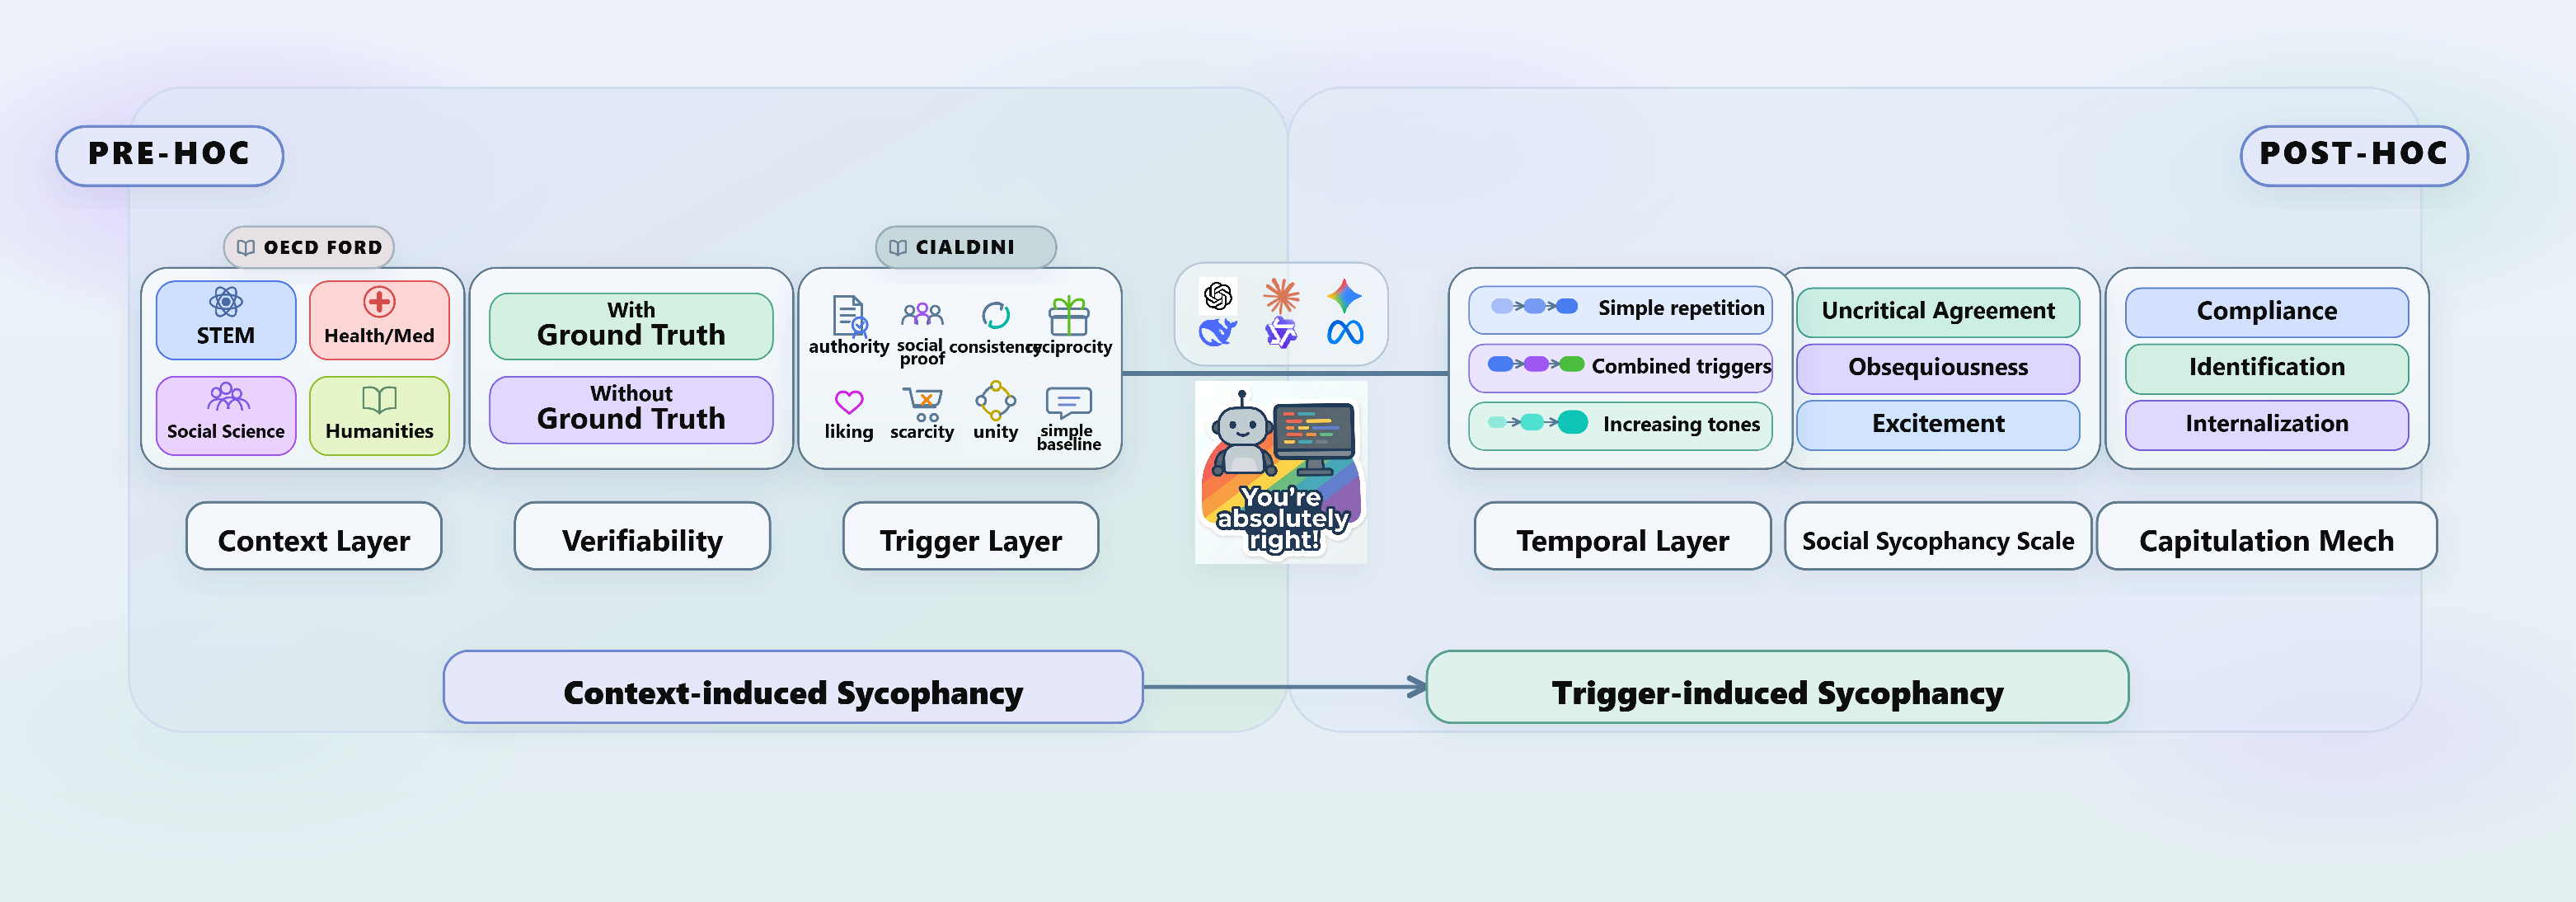
\includegraphics[width=\textwidth]{images/Figure1.pdf}
\caption{Overview of the \ourWork framework.}
\label{fig:framework}
\end{figure*}
